\section{Lecture 16 (May 7th)}
\begin{rmk}
(Liquefaction of gases) If you want to make something really cold, you normally don't just stick it into a refrigerator – instead you put it on dry ice, immerse it in liquid nitrogen, or even liquid helium. These gases are liquefied in the first place using a throttling process.
\end{rmk}
\vspace{2ex}
{\bf Chapter 5}\hspace{2ex}Free Energy and Chemical Thermodynamics
\\\\
{\bf Chapter 5.1}\hspace{2ex}Free Energy and Available Work
\\\\
\begin{defi}
(Free energies) There is Helmholtz free energy $F$ and Gibbs free energy $G$.
\[\begin{cases}
F=U-TS\\
G=H-TS=U+PV-TS
\end{cases}\]
At constant $T$, we can think of these energies as quantities that are minimised as $\Delta V=0$ and $\Delta P=0$ respectively.
\begin{figure}[h!]
\centering
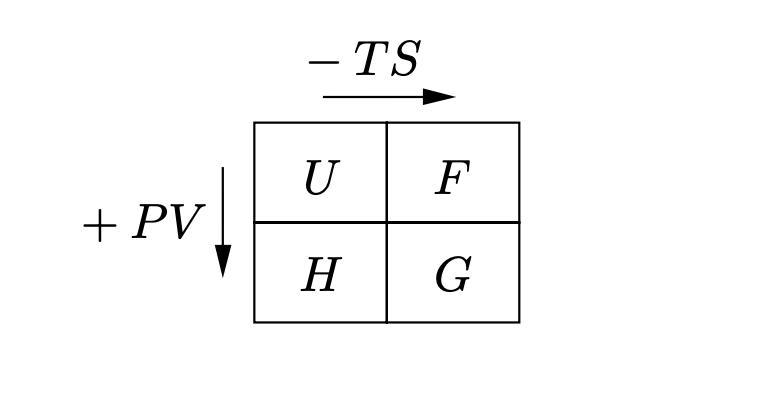
\includegraphics[width=70mm]{FIG1.png}    
\end{figure}
\end{defi}
\vspace{2ex}
\begin{proof}
At constant $T$,
\[\Delta F=\Delta U-T\Delta S=Q+W-T\Delta S\]
Since $T\Delta S\geq Q$, we have $\Delta F\leq W$. On the other hand,
\[\Delta G=\Delta U-T\Delta S+P\Delta V=Q+W-T\Delta S+P\Delta V\]
Since $T\Delta S\geq Q$, we have $\Delta G\leq W$. Therefore, in each case, we see the difference in free energies to be less than the work done by an external system. 
\end{proof}
\vspace{2ex}

